\documentclass[9pt]{beamer}
\setbeamertemplate{caption}[numbered]
\usetheme[white]{Illinois}
%\title[short title]{long title}
\title[HALEU Transitions]{Impacts of Using HALEU on the front end of 
the Nuclear Fuel Cycle}
\subtitle{Good Energy Collective}
\author[Amanda M. Bachmann]{Amanda M. Bachmann\\ Advanced Reactors and Fuel Cycles Group}
%\author[Kathryn D. Huff]{Kathryn D. Huff\\Advanced Reactors and Fuel Cycles Group}
\date[04.29.2022]{April 29, 2022}
\institute[UIUC]{University of Illinois at Urbana-Champaign}


%\usepackage{bbding}
\usepackage{amsfonts}
\usepackage{amsmath}
\usepackage{xspace}
\usepackage{graphicx}
\usepackage{subfigure}
\usepackage{booktabs} % nice rules for tables
\usepackage{microtype} % if using PDF
\usepackage{bigints}
%\usepackage{minted}

\newcommand{\units}[1] {\:\text{#1}}%
\newcommand{\SN}{S$_N$}%{S$_\text{N}$}%{$S_N$}%
\newcommand{\Cyclus}{\textsc{Cyclus}\xspace} %
\newcommand{\Cycamore}{\textsc{Cycamore}\xspace} %
\DeclareMathOperator{\erf}{erf}
%I need some complimentary error funcitons... 
\DeclareMathOperator{\erfc}{erfc}
%Those icons in the references are terrible looking
\setbeamertemplate{bibliography item}[text]

%%%% Acronym support

\usepackage[acronym,toc]{glossaries}
\newacronym[longplural={metric tons of heavy metal}]{MTHM}{MTHM}{metric ton of heavy metal}
\newacronym{ABM}{ABM}{agent-based modeling}
\newacronym{ACDIS}{ACDIS}{Program in Arms Control \& Domestic and International Security}
\newacronym{AHTR}{AHTR}{Advanced High Temperature Reactor}
\newacronym{ANDRA}{ANDRA}{Agence Nationale pour la gestion des D\'echets RAdioactifs, the French National Agency for Radioactive Waste Management}
\newacronym{ANL}{ANL}{Argonne National Laboratory}
\newacronym{API}{API}{application programming interface}
\newacronym{ARCH}{ARCH}{autoregressive conditional heteroskedastic}
\newacronym{ARE}{ARE}{Aircraft Reactor Experiment}
\newacronym{ARFC}{ARFC}{Advanced Reactors and Fuel Cycles}
\newacronym{ARMA}{ARMA}{autoregressive moving average}
\newacronym{ASME}{ASME}{American Society of Mechanical Engineers}
\newacronym{ATWS}{ATWS}{Anticipated Transient Without Scram}
\newacronym{BDBE}{BDBE}{Beyond Design Basis Event}
\newacronym{BIDS}{BIDS}{Berkeley Institute for Data Science}
\newacronym{BOL}{BOL}{Beginning-of-Life}
\newacronym{BSD}{BSD}{Berkeley Software Distribution}
\newacronym{CAFCA}{CAFCA}{ Code for Advanced Fuel Cycles Assessment }
\newacronym{CASL}{CASL}{Consortium for Advanced Simulation of Light Water Reactors}
\newacronym{CDTN}{CDTN}{Centro de Desenvolvimento da Tecnologia Nuclear}
\newacronym{CEA}{CEA}{Commissariat \`a l'\'Energie Atomique et aux \'Energies Alternatives}
\newacronym{CI}{CI}{continuous integration}
\newacronym{CNEC}{CNEC}{Consortium for Nonproliferation Enabling Capabilities}
\newacronym{CNEN}{CNEN}{Comiss\~{a}o Nacional de Energia Nuclear}
\newacronym{CNERG}{CNERG}{Computational Nuclear Engineering Research Group}
\newacronym{COSI}{COSI}{Commelini-Sicard}
\newacronym{COTS}{COTS}{commercial, off-the-shelf}
\newacronym{CSNF}{CSNF}{commercial spent nuclear fuel}
\newacronym{CTAH}{CTAHs}{Coiled Tube Air Heaters}
\newacronym{CUBIT}{CUBIT}{CUBIT Geometry and Mesh Generation Toolkit}
\newacronym{CURIE}{CURIE}{Centralized Used Fuel Resource for Information Exchange}
\newacronym{DAG}{DAG}{directed acyclic graph}
\newacronym{DANESS}{DANESS}{Dynamic Analysis of Nuclear Energy System Strategies}
\newacronym{DBE}{DBE}{Design Basis Event}
\newacronym{DESAE}{DESAE}{Dynamic Analysis of Nuclear Energy Systems Strategies}
\newacronym{DHS}{DHS}{Department of Homeland Security}
\newacronym{DOE}{DOE}{Department of Energy}
\newacronym{DRACS}{DRACS}{Direct Reactor Auxiliary Cooling System}
\newacronym{DRE}{DRE}{dynamic resource exchange}
\newacronym{DSNF}{DSNF}{DOE spent nuclear fuel}
\newacronym{DYMOND}{DYMOND}{Dynamic Model of Nuclear Development }
\newacronym{EBS}{EBS}{Engineered Barrier System}
\newacronym{EDZ}{EDZ}{Excavation Disturbed Zone}
\newacronym{EIA}{EIA}{U.S. Energy Information Administration}
\newacronym{EPA}{EPA}{Environmental Protection Agency}
\newacronym{EP}{EP}{Engineering Physics}
\newacronym{FCO}{FCO}{Fuel Cycle Options}
\newacronym{FCT}{FCT}{Fuel Cycle Technology}
\newacronym{FCWMD}{FCWMD}{Fuel Cycle and Waste Management Division}
\newacronym{FEHM}{FEHM}{Finite Element Heat and Mass Transfer}
\newacronym{FEPs}{FEPs}{Features, Events, and Processes}
\newacronym{FHR}{FHR}{Fluoride-Salt-Cooled High-Temperature Reactor}
\newacronym{FLiBe}{FLiBe}{Fluoride-Lithium-Beryllium}
\newacronym{GCAM}{GCAM}{Global Change Assessment Model}
\newacronym{GDSE}{GDSE}{Generic Disposal System Environment}
\newacronym{GDSM}{GDSM}{Generic Disposal System Model}
\newacronym{GENIUSv1}{GENIUSv1}{Global Evaluation of Nuclear Infrastructure Utilization Scenarios, Version 1}
\newacronym{GENIUSv2}{GENIUSv2}{Global Evaluation of Nuclear Infrastructure Utilization Scenarios, Version 2}
\newacronym{GENIUS}{GENIUS}{Global Evaluation of Nuclear Infrastructure Utilization Scenarios}
\newacronym{GPAM}{GPAM}{Generic Performance Assessment Model}
\newacronym{GRSAC}{GRSAC}{Graphite Reactor Severe Accident Code}
\newacronym{GUI}{GUI}{graphical user interface}
\newacronym{HALEU}{HALEU}{High Assay Low Enriched Uranium}
\newacronym{HEU}{HEU}{High Enriched Uranium}
\newacronym{HLW}{HLW}{high level waste}
\newacronym{HPC}{HPC}{high-performance computing}
\newacronym{HTC}{HTC}{high-throughput computing}
\newacronym{HTGR}{HTGR}{High Temperature Gas-Cooled Reactor}
\newacronym{IAEA}{IAEA}{International Atomic Energy Agency}
\newacronym{IEMA}{IEMA}{Illinois Emergency Mangament Agency}
\newacronym{INL}{INL}{Idaho National Laboratory}
\newacronym{IPRR1}{IRP-R1}{Instituto de Pesquisas Radioativas Reator 1}
\newacronym{IRP}{IRP}{Integrated Research Project}
\newacronym{ISFSI}{ISFSI}{Independent Spent Fuel Storage Installation}
\newacronym{ISRG}{ISRG}{Independent Student Research Group}
\newacronym{JFNK}{JFNK}{Jacobian-Free Newton Krylov}
\newacronym{LANL}{LANL}{Los Alamos National Laboratory}
\newacronym{LBNL}{LBNL}{Lawrence Berkeley National Laboratory}
\newacronym{LCOE}{LCOE}{levelized cost of electricity}
\newacronym{LDRD}{LDRD}{laboratory directed research and development}
\newacronym{LEU}{LEU}{Low Enriched Uranium}
\newacronym{LFR}{LFR}{Lead-Cooled Fast Reactor}
\newacronym{LGPL}{LGPL}{Lesser GNU Public License}
\newacronym{LLNL}{LLNL}{Lawrence Livermore National Laboratory}
\newacronym{LMFBR}{LMFBR}{Liquid-Metal-cooled Fast Breeder Reactor}
\newacronym{LOFC}{LOFC}{Loss of Forced Cooling}
\newacronym{LOHS}{LOHS}{Loss of Heat Sink}
\newacronym{LOLA}{LOLA}{Loss of Large Area}
\newacronym{LP}{LP}{linear program}
\newacronym{LWR}{LWR}{Light Water Reactor}
\newacronym{MARKAL}{MARKAL}{MARKet and ALlocation}
\newacronym{MA}{MA}{minor actinide}
\newacronym{MCNP}{MCNP}{Monte Carlo N-Particle code}
\newacronym{MILP}{MILP}{mixed-integer linear program}
\newacronym{MIT}{MIT}{the Massachusetts Institute of Technology}
\newacronym{MMR}{MMR}{Micro Modular Reactor}
\newacronym{MOAB}{MOAB}{Mesh-Oriented datABase}
\newacronym{MOOSE}{MOOSE}{Multiphysics Object-Oriented Simulation Environment}
\newacronym{MOX}{MOX}{mixed oxide}
\newacronym{MSBR}{MSBR}{Molten Salt Breeder Reactor}
\newacronym{MSRE}{MSRE}{Molten Salt Reactor Experiment}
\newacronym{MSR}{MSR}{Molten Salt Reactor}
\newacronym{NAGRA}{NAGRA}{National Cooperative for the Disposal of Radioactive Waste}
\newacronym{NCSA}{NCSA}{National Center for Supercomputing Applications}
\newacronym{NEAMS}{NEAMS}{Nuclear Engineering Advanced Modeling and Simulation}
\newacronym{NEUP}{NEUP}{Nuclear Energy University Programs}
\newacronym{NFCSim}{NFCSim}{Nuclear Fuel Cycle Simulator}
\newacronym{NFC}{NFC}{Nuclear Fuel Cycle}
\newacronym{NGNP}{NGNP}{Next Generation Nuclear Plant}
\newacronym{NMWPC}{NMWPC}{Nuclear MW Per Capita}
\newacronym{NNSA}{NNSA}{National Nuclear Security Administration}
\newacronym{NPRE}{NPRE}{Department of Nuclear, Plasma, and Radiological Engineering}
\newacronym{NQA1}{NQA-1}{Nuclear Quality Assurance - 1}
\newacronym{NRC}{NRC}{Nuclear Regulatory Commission}
\newacronym{NSF}{NSF}{National Science Foundation}
\newacronym{NSSC}{NSSC}{Nuclear Science and Security Consortium}
\newacronym{NUWASTE}{NUWASTE}{Nuclear Waste Assessment System for Technical Evaluation}
\newacronym{NWF}{NWF}{Nuclear Waste Fund}
\newacronym{NWTRB}{NWTRB}{Nuclear Waste Technical Review Board}
\newacronym{OCRWM}{OCRWM}{Office of Civilian Radioactive Waste Management}
\newacronym{ORION}{ORION}{ORION}
\newacronym{ORNL}{ORNL}{Oak Ridge National Laboratory}
\newacronym{PARCS}{PARCS}{Purdue Advanced Reactor Core Simulator}
\newacronym{PBAHTR}{PB-AHTR}{Pebble Bed Advanced High Temperature Reactor}
\newacronym{PBFHR}{PB-FHR}{Pebble-Bed Fluoride-Salt-Cooled High-Temperature Reactor}
\newacronym{PEI}{PEI}{Peak Environmental Impact}
\newacronym{PH}{PRONGHORN}{PRONGHORN}
\newacronym{PI}{PI}{Principal Investigator}
\newacronym{PNNL}{PNNL}{Pacific Northwest National Laboratory}
\newacronym{PRIS}{PRIS}{Power Reactor Information System}
\newacronym{PRKE}{PRKE}{Point Reactor Kinetics Equations}
\newacronym{PSPG}{PSPG}{Pressure-Stabilizing/Petrov-Galerkin}
\newacronym{PWAR}{PWAR}{Pratt and Whitney Aircraft Reactor}
\newacronym{PWR}{PWR}{Pressurized Water Reactor}
\newacronym{PyNE}{PyNE}{Python toolkit for Nuclear Engineering}
\newacronym{PyRK}{PyRK}{Python for Reactor Kinetics}
\newacronym{QA}{QA}{quality assurance}
\newacronym{RDD}{RD\&D}{Research Development and Demonstration}
\newacronym{RD}{R\&D}{Research and Development}
\newacronym{RELAP}{RELAP}{Reactor Excursion and Leak Analysis Program}
\newacronym{RIA}{RIA}{Reactivity Insertion Accident}
\newacronym{RIF}{RIF}{Region-Institution-Facility}
\newacronym{SAM}{SAM}{Simulation and Modeling}
\newacronym{SCF}{SCF}{Software Carpentry Foundation}
\newacronym{SFR}{SFR}{Sodium-Cooled Fast Reactor}
\newacronym{SINDAG}{SINDA{\textbackslash}G}{Systems Improved Numerical Differencing Analyzer $\backslash$ Gaski}
\newacronym{SKB}{SKB}{Svensk K\"{a}rnbr\"{a}nslehantering AB}
\newacronym{SMR}{SMR}{Small Modular Reactor}
\newacronym{SNF}{SNF}{spent nuclear fuel}
\newacronym{SNL}{SNL}{Sandia National Laboratory}
\newacronym{SNM}{SNM}{Special Nuclear Material}
\newacronym{STC}{STC}{specific temperature change}
\newacronym{SUPG}{SUPG}{Streamline-Upwind/Petrov-Galerkin}
\newacronym{SWF}{SWF}{Separations and Waste Forms}
\newacronym{SWU}{SWU}{Separative Work Unit}
\newacronym{SandO}{S\&O}{Signatures and Observables}
\newacronym{THW}{THW}{The Hacker Within}
\newacronym{TRIGA}{TRIGA}{Training Research Isotope General Atomic}
\newacronym{TRISO}{TRISO}{Tristructural Isotropic}
\newacronym{TSM}{TSM}{Total System Model}
\newacronym{TSPA}{TSPA}{Total System Performance Assessment for the Yucca Mountain License Application}
\newacronym{UDB}{UDB}{Unified Database}
\newacronym{UFD}{UFD}{Used Fuel Disposition}
\newacronym{UML}{UML}{Unified Modeling Language}
\newacronym{UNFSTANDARDS}{UNFST\&DARDS}{Used Nuclear Fuel Storage, Transportation \& Disposal Analysis Resource and Data System}
\newacronym{USNC}{USNC}{Ultra Safe Nuclear Corporation}
\newacronym{UOX}{UOX}{uranium oxide}
\newacronym{UQ}{UQ}{uncertainty quantification}
\newacronym{US}{US}{United States}
\newacronym{UW}{UW}{University of Wisconsin}
\newacronym{VISION}{VISION}{the Verifiable Fuel Cycle Simulation Model}
\newacronym{VV}{V\&V}{verification and validation}
\newacronym{WIPP}{WIPP}{Waste Isolation Pilot Plant}
\newacronym{YMG}{YMG}{Young Members Group}
\newacronym{YMR}{YMR}{Yucca Mountain Repository Site}
\newacronym{NEI}{NEI}{Nuclear Energy Institute}
%\newacronym{<++>}{<++>}{<++>}
%\newacronym{<++>}{<++>}{<++>}


\usepackage{tikz}
\usetikzlibrary{shapes.geometric, arrows, backgrounds}
\usetikzlibrary{positioning, arrows, decorations, shapes}

\tikzstyle{agent} = [rectangle, rounded corners, minimum width=0.1cm, minimum height=0.2cm,text centered, draw=black, fill=blue!30]
\tikzstyle{transition} = [rectangle, rounded corners, minimum width=0.1cm, minimum height=0.2cm,text centered, draw=black, fill=red!30]
\tikzstyle{arrow} = [thick,->,>=stealth]

\tikzstyle{region} = [rectangle, rounded corners, minimum width=0.1cm, minimum height=0.2cm,text centered, draw=black, fill=green!30]
\tikzstyle{institution} = [rectangle, rounded corners, minimum width=0.1cm, minimum height=0.2cm,text centered, draw=black, fill=red!30]
\tikzstyle{facility} = [rectangle, rounded corners, minimum width=0.1cm, minimum height=0.2cm,text centered, draw=black, fill=blue!30]
\tikzstyle{connect} = [thick,-]

\def\firstcircle{(0,0) circle (2cm)}
\def\secondcircle{(60:3cm) circle (2cm)}
\def\thirdcircle{(0:3cm) circle (2cm)}
\makeglossaries

%try to get rid of header on title page\dots
\makeatletter
    \newenvironment{withoutheadline}{
        \setbeamertemplate{headline}[default]
        \def\beamer@entrycode{\vspace*{-\headheight}}
    }{}
\makeatother

\makeatother
\setbeamertemplate{footline}
{
  \leavevmode%
  \hbox{%
    \rightline{\insertframenumber{} / \inserttotalframenumber\hspace*{1ex}}
  }%
  \vskip0pt%
}
\makeatletter
\begin{document}
%%%%%%%%%%%%%%%%%%%%%%%%%%%%%%%%%%%%%%%%%%%%%%%%%%%%%%%%%%%%%
%% From uw-beamer Here's a handy bit of code to place at 
%% the beginning of your presentation (after \begin{document}):
\newcommand*{\alphabet}{ABCDEFGHIJKLMNOPQRSTUVWXYZabcdefghijklmnopqrstuvwxyz}
\newlength{\highlightheight}
\newlength{\highlightdepth}
\newlength{\highlightmargin}
\setlength{\highlightmargin}{2pt}
\settoheight{\highlightheight}{\alphabet}
\settodepth{\highlightdepth}{\alphabet}
\addtolength{\highlightheight}{\highlightmargin}
\addtolength{\highlightdepth}{\highlightmargin}
\addtolength{\highlightheight}{\highlightdepth}
\newcommand*{\Highlight}{\rlap{\textcolor{HighlightBackground}{\rule[-\highlightdepth]{\linewidth}{\highlightheight}}}}
%%%%%%%%%%%%%%%%%%%%%%%%%%%%%%%%%%%%%%%%%%%%%%%%%%%%%%%%%%%%%
%%--------------------------------%%
\begin{withoutheadline}
    \frame{
      \titlepage
    }
    \end{withoutheadline}

%%--------------------------------%%
\AtBeginSection[]{
\begin{frame}
  \frametitle{Outline}
  \tableofcontents[currentsection]
\end{frame}
}

\begin{frame}
    \frametitle{Acknowledgements}
    This material is based upon work supported under an Integrated University 
Program Graduate Fellowship. Any opinions, findings, conclusions, or 
recommendations expressed in this publication are those of the author(s) 
and do not necessarily reflect the views of the Department of Energy Office 
of Nuclear Energy.

    \begin{block}{Disclaimer}
        None of the results presented in this presentation have been 
        published and have not been peer reviewed. 
        
    \end{block}

\end{frame}
\section{Introduction \& Objectives}
\begin{frame}
    \frametitle{Introduction}
    \begin{columns}
        \column[t]{5cm}
    \begin{itemize}
    \item Multiple new reactor designs require \gls{HALEU} fuel, which allows for: 
    \begin{itemize}
        \item Longer cycle times
        \item Higher burnups 
    \end{itemize}
    \item<1-> To meet the \gls{HALEU} demand, the U.S. \gls{DOE} has proposed two methods \cite{griffith_overview_2020}:
    \begin{itemize}
        \item Recovery and downblending of \gls{HEU}
        \item Enrichment of natural uranium
    \end{itemize}
    \end{itemize}

    \column[t]{5cm}
    \begin{table}
        \centering
        \caption{Categories of uranium enrichment by weight fraction of 
        uranium-235.}
        \label{tab:enrichemnt}
        \begin{tabular}{l c c}
            \hline
            Category & Weight fraction (\%)\\\hline
            Depleted & $<$0.711 \\
            Natural & 0.711 \\
            LEU & 0.711-20 \\
            \gls{HALEU} & 5-20 \\
            \gls{HEU} & $\ge$20 \\
            \hline
        \end{tabular}
    \end{table}
    \end{columns}
\end{frame}

\begin{frame}
    \frametitle{Overview of the Nuclear Fuel Cycle}
    \begin{figure}[t]
    \centering
    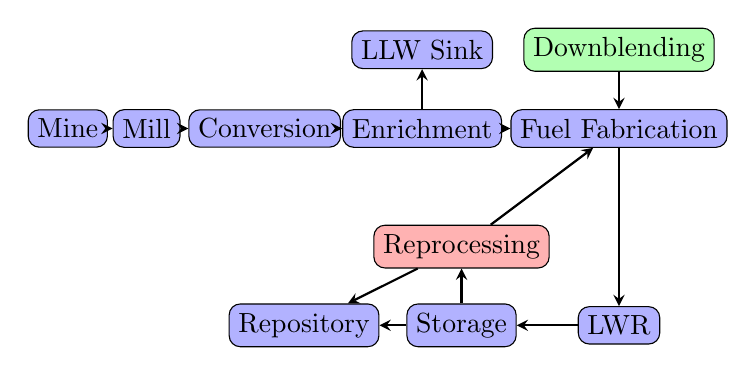
\begin{tikzpicture}[node distance=1cm]
        \node (mine) [agent] {Mine};
        \node (mill) [agent, right of=mine] {Mill};
        \node (conversion) [agent, right of=mill, xshift=0.5cm] {Conversion};
        \node (enrichment) [agent, right of=conversion, xshift=1cm]{Enrichment};
        \node (fabrication) [agent, right of=enrichment, xshift=1.5cm]{Fuel Fabrication};
        \node (reactor) [agent, below of=fabrication, yshift=-1.5cm]{LWR};
        \node (storage) [agent,  left of=reactor, xshift=-1cm]{Storage};
        \node (sinkhlw) [agent, left of=storage, xshift=-1cm]{Repository};
        \node (sinkllw) [agent, above of=enrichment]{LLW Sink};


        \draw [arrow] (mine) --  (mill); 
        \draw [arrow] (mill) -- (conversion); 
        \draw [arrow] (conversion) -- (enrichment);
        \draw [arrow] (enrichment) -- (fabrication);
        \draw [arrow] (enrichment) -- (sinkllw);
        \draw [arrow] (fabrication) -- (reactor);
        \draw [arrow] (reactor) -- (storage);
        \draw [arrow] (storage) -- (sinkhlw);
        \pause
        \node (reprocessing) [transition, above of=storage]{Reprocessing};
        
        \draw [arrow] (storage) -- (reprocessing);
        \draw [arrow] (reprocessing) -- (fabrication);
        \draw [arrow] (reprocessing) -- (sinkhlw);
        \pause
        \node (downblending) [region, above of=fabrication]{Downblending};
        \draw [arrow] (downblending) -- (fabrication);

        \end{tikzpicture}
    \caption{Overview of the Nuclear Fuel Cycle.}
    \label{fig:fuel_cycle}
\end{figure}
\end{frame}

\begin{frame}
    \frametitle{Objectives}
    This work explores how developing a supply chain of \gls{HALEU} affects 
    the nuclear fuel cycle in the US. 
    Quantify material requirements of the transition to reactors 
              fueled by \gls{HALEU}
    \begin{itemize}
        \item<-1> The number of reactors deployed 
        \item<-1> Mass of enriched uranium sent to reactors
        \item<-1> Mass of feed uranium required to produce enriched uranium
        \item<-1> \gls{SWU} capacity required to enrich uranium 
    \end{itemize}
\end{frame}
\section{Transition Analysis}
\begin{frame}
    \frametitle{Once-through transitions provide expected demand of \gls{HALEU}}
        \begin{itemize}
            \item If we understand the demand for \gls{HALEU} for reactors, 
            then we can understand how much needs to be made and how that 
            demand affects the rest of the fuel cycle. 
            \pause
            \item Factors that affect demand:
            \begin{itemize}
                \item Reactor type
                \item Energy demand
            \end{itemize}
            \pause
            \item We can use fuel cycle simulators to model these transitions
        \end{itemize}
\end{frame}

\begin{frame}
    \frametitle{Fuel cycle models contains various assumptions}
    \begin{columns}
        
    \column[t]{6cm}
    \vspace{-0.9cm}
    \begin{figure}[t]
    \centering
    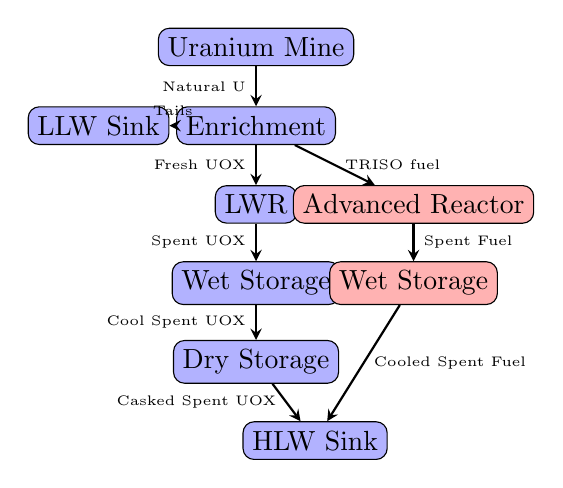
\begin{tikzpicture}[node distance=1cm]
        \node (mine) [agent] {Uranium Mine};
        \node (enrichment) [agent, below of=mine]{Enrichment};
        \node (reactor) [agent, below of=enrichment]{LWR};
        \node (adv_reactor) [transition, below of=enrichment, xshift=2cm]{Advanced Reactor};
        \node (wetstorage) [agent, below of=reactor]{Wet Storage};
        \node (drystorage) [agent, below of=wetstorage]{Dry Storage};
        \node (sinkhlw) [agent, below of=drystorage, xshift=0.75cm]{HLW Sink};
        \node (sinkllw) [agent, left of=enrichment,xshift=-1cm]{LLW Sink};
        \node (adv_rx_cooling) [transition, below of=adv_reactor]{Wet Storage};

        \draw [arrow] (mine) -- node[anchor=east]{\tiny Natural U} (enrichment); 
        \draw [arrow] (enrichment) -- node[anchor=south]{\tiny Tails}(sinkllw);
        \draw [arrow] (enrichment) -- node[anchor=east]{\tiny Fresh UOX}(reactor);
        \draw [arrow] (enrichment) -- node[anchor=west]{\tiny TRISO fuel}(adv_reactor);
        \draw [arrow] (reactor) -- node[anchor=east]{\tiny Spent UOX}(wetstorage);
        \draw [arrow] (wetstorage) -- node[anchor=east]{\tiny Cool Spent UOX}(drystorage);
        \draw [arrow] (drystorage) -- node[anchor=east]{\tiny Casked Spent UOX}(sinkhlw);
        \draw [arrow] (adv_reactor) -- node[anchor=west]{\tiny Spent Fuel}(adv_rx_cooling);
        \draw [arrow] (adv_rx_cooling) -- node[anchor=west]{\tiny Cooled Spent Fuel}(sinkhlw);
        \end{tikzpicture}
    \caption{Fuel cycle facilities and material flow between facilities. Facilities 
    in red are deployed after 2025 for the transition. }
    \label{fig:fuel_cycle}
\end{figure}

        \column[t]{4.5cm}
        Model transitions using \Cyclus \cite{huff_fundamental_2016}
    \begin{itemize}
        \item Simulations model reactor deployment from 1965-2090
        \item<2-> \gls{LWR} commission dates are obtained from the IAEA PRIS
              database \cite{noauthor_power_1989}
        \item<2-> \glspl{LWR} are assumed to operate until their current license 
              expires
        \item<3-> Transitions begin in 2025
        \item<3-> \Cyclus determines the number of reactors that need to be deployed
    \end{itemize}

\end{columns}
\end{frame}

\begin{frame}
    \frametitle{Multiple reactors and energy demands are considered}
    \begingroup
        \renewcommand{\arraystretch}{-0.5}
        \vspace{-0.4cm}
        \begin{table}
            \small
            \caption{Advanced reactor design specifications}
            \label{tab:reactor_summary}
            \begin{tabular}{ c c c c }
                \hline
                Design Criteria & USNC MMR 
                    \cite{mitchell_usnc_2020} & 
                    X-energy Xe-100 \cite{harlan_x-energy_2018,hussain_advances_2018} & 
                    VOYGR \cite{nuscale_chapter_2020,nuscale_chapter_2020-1}\\\hline
                Power Output (MWe) & 10 & 75 & 50\\
                Enrichment (\% $^{235}U$) & 13 & 15.5 & 4.09 \\
                Cycle Length (yr) & 20 & Online & 2 \\
                Reactor Lifetime (yr) & 20 & 60 & 60\\
                Burnup ($\frac{MWd}{kg U}$) & 42.7 & 160 & 36\\
                \hline
            \end{tabular}
        \end{table}   
        \endgroup
        \pause
        \begin{table}[ht]
            \centering
            \caption{Summary of the once-through fuel cycle transition scenarios.}
            \label{tab:scenarios_once-through}
            \begin{tabular}{c l l}
                    \hline
                    Scenario number & Reactors present & Energy growth model\\\hline
                    1 & \glspl{LWR} & N/A \\
                    2 & \glspl{LWR} and \gls{MMR} & No growth \\
                    3 & \glspl{LWR} and Xe-100 & No growth \\
                    4 & \glspl{LWR}, Xe-100, and \gls{MMR}& No growth\\
                    5 & \glspl{LWR}, \gls{MMR}, and VOYGR & No growth\\
                    6 & \glspl{LWR}, Xe-100, and VOYGR & No growth\\
                    7 & \glspl{LWR}, Xe-100, \gls{MMR}, and VOYGR & No growth\\
                    \hline
            \end{tabular}
        \end{table}
    

\end{frame}
\section{Ongoing Work}
\begin{frame}
      \frametitle{Ongoing Work}
        \begin{columns}
          \column[t]{4.5cm}
            \begin{itemize}
            \item Once-through transitions
              \begin{itemize}
                  \item Incorporate \gls{LWR} license expiration dates
                  \item Quantify natual uranium needs and waste production 
                        in these transitions
                  \item Simulate transitions to multiple types of advanced reactors
              \end{itemize}
            \pause
            \item Model transitions with recycling
            \begin{itemize}
              \item Impacts the resource utilization?
              \item Impacts of limited vs continuous 
                    recycling?
            \end{itemize}
          \end{itemize}

          \column[t]{6cm}
          \begin{figure}
    \centering
    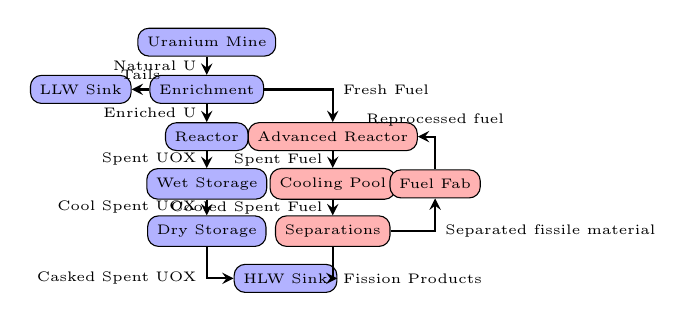
\begin{tikzpicture}[node distance=0.6cm]
        \node (mine) [facility] {\tiny Uranium Mine};
        \node (enrichment) [facility, below of=mine]{\tiny Enrichment};
        \node (reactor) [facility, below of=enrichment]{\tiny Reactor};
        \node (adv_reactor) [transition, right of=reactor, xshift=1cm]{\tiny Advanced Reactor};
        \node (wetstorage) [facility, below of=reactor]{\tiny Wet Storage};
        \node (drystorage) [facility, below of=wetstorage]{\tiny Dry Storage};
        \node (cooling) [transition, below of=adv_reactor]{\tiny Cooling Pool};
        \node (sinkhlw) [facility, below of=drystorage, xshift=1cm]{\tiny HLW Sink};
        \node (sinkllw) [facility, left of=enrichment, xshift=-1cm]{\tiny LLW Sink};
        \node (separation) [transition, below of=cooling]{\tiny Separations};
        \node (fuelfab) [transition, below of=adv_reactor,xshift=1.3cm]{\tiny Fuel Fab};

        \draw [arrow] (mine) -- node[anchor=east]{\tiny Natural U} (enrichment);
        \draw [arrow] (enrichment) -- node[anchor=east]{\tiny Enriched U}(reactor);
        \draw [arrow] (enrichment) -- node[anchor=south]{\tiny Tails}(sinkllw);
        \draw [arrow] (enrichment) -| node[anchor=west]{\tiny Fresh Fuel}(adv_reactor);
        \draw [arrow] (reactor) -- node[anchor=east]{\tiny Spent UOX}(wetstorage);
        \draw [arrow] (wetstorage) -- node[anchor=east]{\tiny Cool Spent UOX}(drystorage);
        \draw [arrow] (drystorage) |- node[anchor=east]{\tiny Casked Spent UOX}(sinkhlw);
        \draw [arrow] (adv_reactor) -- node[anchor=east]{\tiny Spent Fuel}(cooling);
        \draw [arrow] (cooling) -- node[anchor=east]{\tiny Cooled Spent Fuel}(separation);
        \draw [arrow] (separation) -| node[anchor=west]{\tiny Separated fissile material}(fuelfab);
        \draw [arrow] (fuelfab) |- node[anchor=south]{\tiny Reprocessed fuel}(adv_reactor);
        \draw [arrow] (separation) |- node[anchor=west]{\tiny Fission Products}(sinkhlw);

        \end{tikzpicture}
    \caption{Fuel cycle facilities and material flow between facilities. Facilities in 
    red are added in for the transition scenarios.}
    \label{fig:recycle_fuel_cycle}
\end{figure}
          \end{columns}
\end{frame}

\begin{frame}
  \frametitle{Ongoing Work (Cont.)}
    \begin{itemize}
      \item Perform sensitivity analysis
              \begin{itemize}
                  \item Transition start time
                  \item Fleet share for each reactor
                  \item \gls{LWR} lifetimes
              \end{itemize}
      \item Optimize the transition
            \pause
            \item Investigate neutronics effects of \gls{HEU} impurities
              \begin{itemize}
                  \item Effects on neutron flux and $k_{eff}$
                  \item Effects on safety parameters?
                  \item More work to investigate this question?
              \end{itemize}
    \end{itemize}
\end{frame}



\begin{frame}[allowframebreaks]
    \frametitle{References}
    \bibliographystyle{plain}
    {\footnotesize \bibliography{bibliography} }
  
  \end{frame}
\begin{frame}
    \frametitle{Summary}
    \begin{columns}
      \column[t]{5cm}
      \begin{itemize}
        \item Investigating the transition to \gls{HALEU}-fueled reactors
        \item Results show larger uranium mass requirements to transition to 
              \gls{MMR} than Xe-100
        \item Working on investigation material needs when fuel is recycled.
      \end{itemize}

      \column[t]{5cm}
        \begin{figure}[t]
          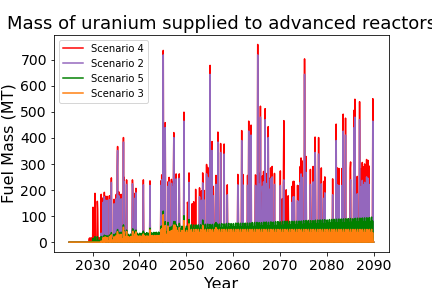
\includegraphics[scale=0.35]{figures/advancedRX_fuelsupply_scenarios_2-5.png}
        \end{figure}
        
    \end{columns}
    
\end{frame}

\end{document}
